\documentclass{entcs} 
\usepackage{CSC8498macro}
\usepackage{graphicx}
\usepackage{float}
\graphicspath{{./Images/}}
%% This document describes the formatting instructions for the CSC8498 final report.

\makeatletter

\def\lastname{Boulderstone}
\begin{document}

\begin{frontmatter}
\title{Rollback Netcode, Implmentation and Adoption}
\author{Edward Boulderstone}
  \address{School of Computing Science, Newcastle University, UK} 
\thanks[nigellemail]{Email:
    \href{mailto:E.Boulderstone@ncl..ac.uk} {\texttt{\normalshape
        E.Boulderstone@ncl..ac.uk}}}

			
				
\begin{abstract} 
Rollback netcode is a process sychronisation method for interactive multi-user games played over a network with latency. The method has the potential to improve online game experiences by minimizing the effects of latency in the networks used by remote gamers. The focus of this project is 'fighting games' where the quality of the game experience is driven by the smoothness and apparent immediacy of the game action. The implementation of rollback netcode in the games industry has been slow and difficult. This project explores the difficulties implementing rollback, and researches optimizations that can be made to existing open source rollback netcode.
\end{abstract}

\begin{keyword}
rollback, netcode, peer to peer, fighting games, networking, industry.
\end{keyword}
\end{frontmatter}

\section{Introduction}\label{sec: introduction}
Multiplayer online games have continued to gain popularity over the last few years as the growth and capacity of the internet has increased. These games allow people from all over the world to effectively play the same game at the same time in the same game environment. However, games that involve fight simulations between players require a level of interaction that has been difficult to achieve on wide area networks. To side-step these network latency issues, many fans of fighting games have gone out of their way to organise local tournaments, with most major tournaments before the pandemic taking place off-line\cite{FGCMajors}. Games where fighting is a central component to the game play has its roots in the video arcades of the mid 1990's,\cite{FirstUSTournament} and continued until the start of the pandemic, in part because fighting games rely on consistent timing and a low latency network environment \cite{DelayVsRollback}, \cite{BadNetcode}. The networking solutions during the early years of the internet simply did not provide an environment for competitive play\cite{FGCAsEsport}. However, with the spread of corona virus in the 2020's, fighting style games had to use the low latency internet for multiuser games. Games which did not have well optimized netcode found themselves at a disadvantage, with reduced attention \cite{SmashTournamentsInThePandemic}, while games with well written netcode found significantly more success  \cite{GuiltyGearStriveInThePandemic}.

\subsection{Delay Based Netcode}
The classic solution to game synchronisation for online multiplayer games is a peer to peer network system known as delay based netcode. Peer to peer netcode is important for fighting games because of the low latency requirement. Most fighting games are between two players \cite{FightingGameDefine}, where the game must maintain state and synchronisation. Delay based netcode works by keeping the two players games synchronised, by exchanging network frames, before updating the game status. In effect, in delay based netcode. A satisfactory game experience can only occur on a very low latency network with this methodology.

\subsection{Rollback Netcode}
Rollback netcode was developed in 2006 as a solution to the problems with delay based netcode. \cite{RollbackDevelopment}. Rollback netcode is underpinned by delay based netcode but also contains rollback features and the prediction of user inputs. As game play progresses, the system predicts the response of the other player(s) to the most recent player action. If the prediction is accurate game play continues. However, if the prediction is incorrect the game will be "rollbacked" to the point where the discrepancy occured; and the game state will be re-simulated back to the real time frame as shown in figure \ref{fig:RollbackNetcodeRepresentation}. The accuracy of the prediction and the method of rollback are clearly critical success factors in making this system function well. Poor prediction will lead to many rollbacks which can produce a jerky game experience.

\begin{figure}[H]
\centering
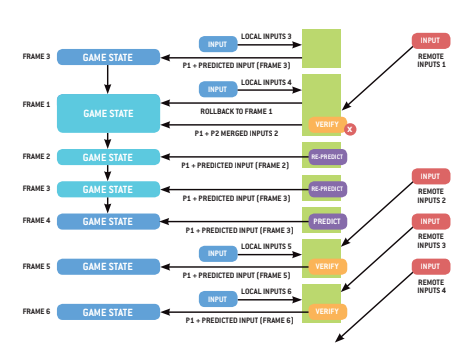
\includegraphics{RollbackNetcodeRepresentation}
\caption{Rollback netcode \cite{GGPODocumentation}}
\label{fig:RollbackNetcodeRepresentation}
\end{figure}
\newpage

\subsection{Rollback Netcode in The Fightgame market}
In today's fighting game market, many games have rollback \cite{GamesWithRollback} implemented to improve the user experience in game play. However there are still notable exceptions such as:
\begin{itemize}
\item Super Smash Bros. Ultimate\cite{SSBU}
\item Granblue Fantasy Versus\cite{GBFV}
\item Under Night In-Birth\cite{UNI}
\item Samurai Shodown\cite{SamSho}
\item Soulcalibur VI\cite{SVI}
\item Dead or Alive 6\cite{DOA6}
\item EA Sports UFC 4\cite{UFC4}
\item Dragon Ball FighterZ\cite{DBFZ}
\end{itemize}

Other fighting games have had difficulty in implementing rollback, such as Street Fighter V and Mortal Kombat X.
These difficulties with implementing and developing rollback are the basis of the motivation of this paper.

\subsection{Aim}
To investigate rollback netcode, it's usage in the game industry and short comings of existing open source rollback netcode software.
\subsection{Objectives}
\begin{itemize}
\item Understand rollback netcode and the effects on the games it's implemented in.
\item Create a visualization for the differences between rollback and delay based netcode.
\item Research the difficulties of implementing rollback in existing games.
\item Explore optimizations for the existing open source rollback software.
\item Investigate further uses of rollback netcode, in the wider video game industry.
\end{itemize}
\newpage
\section{Background}
\subsection{Peer to Peer Netcode}
Peer to peer networks over the internet communicate though data packets. Data packet communication can have the following issues.
\begin{itemize}
\item{Packets take time to reach their destination (Network Latency).}
\item{Packets can get lost through the network (Packet Loss).}
\item{Packets can become corrupted on route (Corruption).}
\item{Computers have different processing capacity and hence process packets at different rates.}
\item{Computers can be busy with other tasks and miss packets.}
\end{itemize}

By reducing the impact of these flaws in data packet communication the user experience of online games can be considerably improved. One overall method to reduce the impact of data packet delay and loss is to set a minimium tolerable connection quality. This minimum tolerable connection quality can be pre-defined, depending on the requirements of the game, and tested for each user as they connect to the online game server. As the selection of players (matchmaking) for a multiuser game is in the control of the game software, players can be matched together who have good network connectivity to each other. 

\subsection{Delay-based netcode}
\subsubsection{Concept}
Delay based netcode works by keeping game players in lockstep, meaning that each player's simulation of the game waits for the input of the other player(s), before simulating the current frame\cite{DelayBasedNetcode}. This system works well when latency is not a major factor, for example, in a turn based games, where the inputs are spread apart by seconds, a pause of half a second may go unnoticed.

Local user input can be delayed by a number of frames to compensate for the Network Latency, as seen in figure \ref{fig:InputLatencyEffect}.

\begin{figure}[H]
\centering
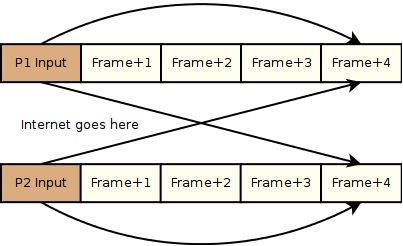
\includegraphics{InputDelay}
\caption{4 Frame Input Delay Example \cite{FightingGameNetworking}}
\label{fig:InputLatencyEffect}
\end{figure}

The Input delay can be calculated as follows:\\

\[InputLatencyFrames = Ceiling( \frac{RoundTripLatency}{2 * FrameDuration} ) + \epsilon\]

Where $\epsilon$ represents additional frames of delay to compensate for variance in Network Latency.

\subsubsection{Improvements To Delay Based Netcode}
However the 4 Frame Input Delay Example does not take into account the potential for packet loss or corrupted packets, which may lead the game states to progress as shown in figure \ref{fig:PacketLossEffect}

\begin{figure}[h]
\centering
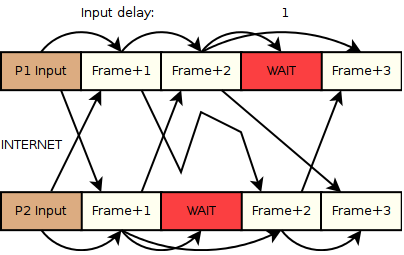
\includegraphics{PacketLossEffect}
\caption{The affect of packet loss on game state progression \cite{FightingGameNetworking}}
\label{fig:PacketLossEffect}
\end{figure}

One further affect of packet loss with single input packets is knock on delays, where a delay in one frame, delays the delivery of subsequent frames. This causes inputs to be lost or delayed resulting in a intermittent user experience.

To combat packet loss and data corruption multiple frames inputs can be sent within one packet, extra frames of input delay can be added, and inputs can be sent multiple times, as shown in figure \ref{fig:PacketLossSoultions}

\begin{figure}[H]
\centering
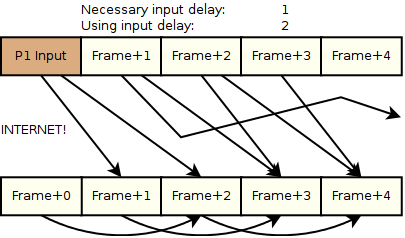
\includegraphics{PacketLossSoultions}
\caption{Potential Solutions to Packet Loss in Delay Based Netcode \cite{FightingGameNetworking}}
\label{fig:PacketLossSoultions}
\end{figure}

Another way to improve delay based netcode is to account for Network Latency variance with a dynamic number of short input delays. These input delays can help to reduce the intermittentcy of the game players synchronized by briefly delaying the action for both of the players while the other player catches up\cite{DelayVsRollback}. This can hide screen stutters, and reduce the impact of degrading network conditions that could cause consistent game pauses. However, data packet delivery consistency for fighting games is a primary determinant of quality of user experience\cite{Core-ARollback}, because of the highly interactive nature of fight simulation.

\subsubsection{Evaluation}
In an environement with minimal Network Latency variance, the delay based netcode has a similar functionality to a non-networked game experience. This is the ideal case for delay based networking. However, when the Network Latency variance is high, the game can freeze at seemingly random moments, removing agency from the player in the middle of a game. This breaks user immersion and significantly decreases the quality of the experience\cite{DelayVsRollback}\cite{KIInterview}.
\subsection{Rollback netcode}
\subsubsection{Concept}
Rollback netcode takes the existing framework of delay based netcode and builds on top of it. Instead of waiting for the remote user's input to simulate a frame, the game predicts it.  The game can then proceed independently for all the users for a short time, In the event a packet is lost or late, the rollback frames act as a buffer preventing the from game freezing. Thus the game is more resilient to turbulent network conditions than delay based netcode \cite{GGPODocumentation}. 

\subsubsection{Extra functionality required to support Rollback Netcode}
Implementing rollback is not as simple as changing the existing networking solution, other factors have to be considered, these include:
\begin{itemize}
\item Decouple gameplay logic from screen rendering
\item Fast storage and retrieval of game state
\item Loadable game state
\item Faster than real time game state simulation
\end{itemize}
\subsubsection{Issues In theory}
Rollback does not require the remote users input to simulate a frame. However rollback has implementation issues.
\begin{itemize}
\item Particle Systems.
A particle system is a technique that uses many minute graphic objects to simulate certain kinds of "fuzzy" phenomena e.g. rain. Particles are computationally expensive to process, and their rollback is complex and difficult.

\item Sound Effects

Typically sound effects are buffered in the audio driver, with limited ability to pause the effect or play from a specific time stamp. Therefore, managing the game sound with rollback particularly problematic.

\item Desync Detection

Desync is the process by which the game state of different users is unreconcilable, so that drastic action has to be taken to continue the game play.  In rollback it is quite often difficult to detect a desync happening as it is expected that the different users have different game states.
\item Optimization
Because rollback can require the simulation of multiple game states in the space of a normal time interval, more processing capacity will be required to implement.
\end{itemize}
\subsection{Comparison}
In comparing rollback netcode vs delay based netcode, a number of factors to be used, the factors chosen in this study are:
\begin{itemize}
\item Simple to implement without complex real time dependant rollback code
\item Visually smooth for more realistic simulation
\item Computationally Performant, the required processing capacity to create a realistic game
\item Robust to network turbulence, computer performance and user interaction
\item Low bandwidth to minimize the amount of network traffic required to support game play.
\item Responsive to user input i.e. the game responds immediately to user commands
\end{itemize}
The analysis of Nether realm studio \cite{8Frames} is that delay based netcode is superior to rollback in the simple, visually smooth and performant categories, whilst the rollback netcode is superior in the responsive category.

As previously discussed responsiveness is critical to fighting game simulation, meaning that rollback is required for this category of games.
\begin{figure}[H]
\centering
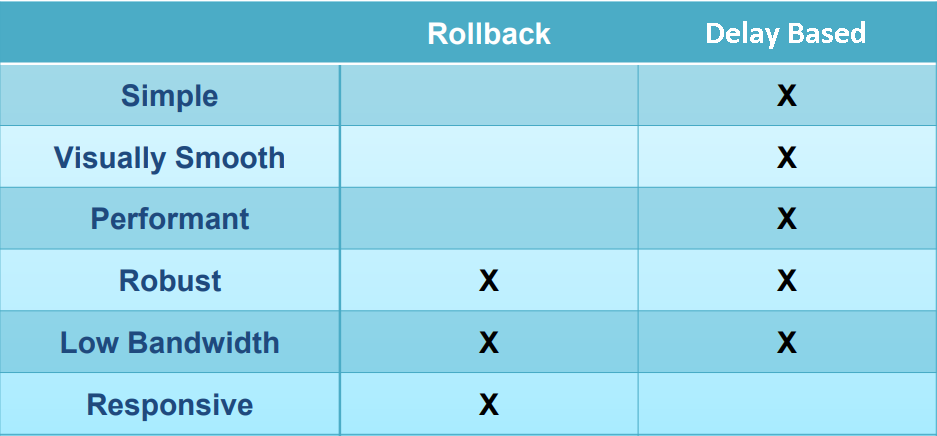
\includegraphics[width=\textwidth]{NetcodeCompare}
\caption{Table comparing differences between Rollback and Delay Based Netcode\cite{8Frames}}
\label{fig:NetcodeCompare}
\end{figure}


\section{Industry Issues}
The fighting game industry has had significant difficulty in adopting rollback netcode into their existing games \ref{sec: introduction}. In this section, Street Fighter V and Mortal Kombat X are analysed, to understand the issues they have had with the implementation of rollback.
\subsection{Street Fighter V}
Street Fighter V(SFV)'s rollback netcode was released to the public to widespread disappointment \cite{Netcode 1} \cite{Netcode 2} \cite {Netcode 3} \cite {Netcode 4} \cite{Core-ARollback}.  The following issues were found with SFV's rollback:
\begin{itemize}
\item One Sided rollback. \cite{SFV 1}  \cite{SFV 2} \cite {SFV 3}
One sided rollback is when two game states drift out of sync, through either a series of lost packets, or one machine failing to keep up with the required frame rate. The effect of this that one user, will have to process a large number of rollbacks. Whilst the other user will not receive fewer rollbacks as shown in figure \ref{fig:OneSided}
\vspace{1em}
\begin{figure}[H]
\resizebox{\textwidth}{!}{
\begin{tabular}{c|c|c|c|c}
\hline
\multicolumn{2}{c|}{User 0} & & \multicolumn{2}{c}{User 1} \\
\hline
Local Frame & Local Network Events & & Local Network Events & Local Frame\\
\hline
0 & Send 0's input for frame 0 && Send 1's input for frame 1 & 0 \\
\hline
1 & Send 0's input for frame 1 && Send 1's input for frame 1(Lost) & 1 \\
1 & Receive 1's input for frame 0 && Receive 0's input for frame 0 & 1 \\
\hline
2 & Send 0's input for frame 2 && Send 1's input for frame 2(Lost) & 2 \\
2 & Guesses 1's input for frame 1 && Receive 0's input for frame 1 & 2 \\
\hline
3 & Send 0's input for frame 3 && Send 1's input for frame 3(Lost) & 3 \\
3 & Halt for 1's input from frame 1 && Receive 0's input for frame 2 & 3 \\
\hline
3 & Send 0's input for frame 3 && Send 1's input for frame 4 & 4 \\
3 & Receive 1's input for frame 1,2 and 3 (Rollback) && Receive 0's input for frame 3 & 4 \\
\hline
4 & Sends 0's input for frame 4 && Sends 1's input for frame 4 & 5 \\
4 & Receive 1's input for frame 4 && Guesses 0's input for frame 3 & 5 \\
\hline
\end{tabular}
}
\caption{A demonstration of how onesided rollback occurs in a network with one frame of input delay and one rollback frame}
\label{fig:OneSided}
\end{figure}
\item Dynamic Delay frames. \cite{SFV 1}
To accomplish rollback netcode in existing SFV, dynamic delay frames have been used.
Dynamic delay frames, which delay action on the user inputs, can make the game feel slow despite not freezing. 
\item The rollback of large effects such as particle and audio effects causes jarring experiences for the user\cite{SFV 1}.
\end{itemize}
There are a number of ways these issues with rollback netcode can be resolved. These include fixing one sided rollback, using static delay frames, and making event are confirmed before large effects are used.

\subsection{Mortal Kombat X}
Mortal Kombat X (MKX) was released in 2015 with delay based netcode. Rollback netcode was added in a patch to the game in 2018. However there are considerable development required to reimplement the game with rollback features.

The lessons learnt from this redevelopment include, defining a network quality threshold so that a maximum of 8 frames would be considered in a rollback scenario. Performance improvements such as:
\begin{itemize}
\item Multithreading
\item During rollback compute predefined object changes, rather than transmit them in a frame update.
\item Only serialize selective game states to maximize performance.
\item Use fuzzy matching on non gameplay effects.
\end{itemize}

\section{Rollback Visualization tool}
To demonstrate the effectiveness of Rollback vs Delay based netcode, a simulation of the two different styles of netcode was produced.
\subsection{Design}
The high level design of this visualization tool was to have two side by side game clients, communicating with each other through simulated latency and netcode. As the visualization tool was designed to be a demonstration, no overly complex mechanics were implemented. The tool consisted of two avatars that could move and jump.

Unity was chosen as the engine to develop the simulation.

The user of the visualization tool has the option to change the properties of the simulated network latency in real time, and the properties of the netcode, such as Input Latency, Rollback frames. 
The overall design of the visualization tool is shown in figure \ref{fig:DFD}.

\begin{figure}[h]
\centering
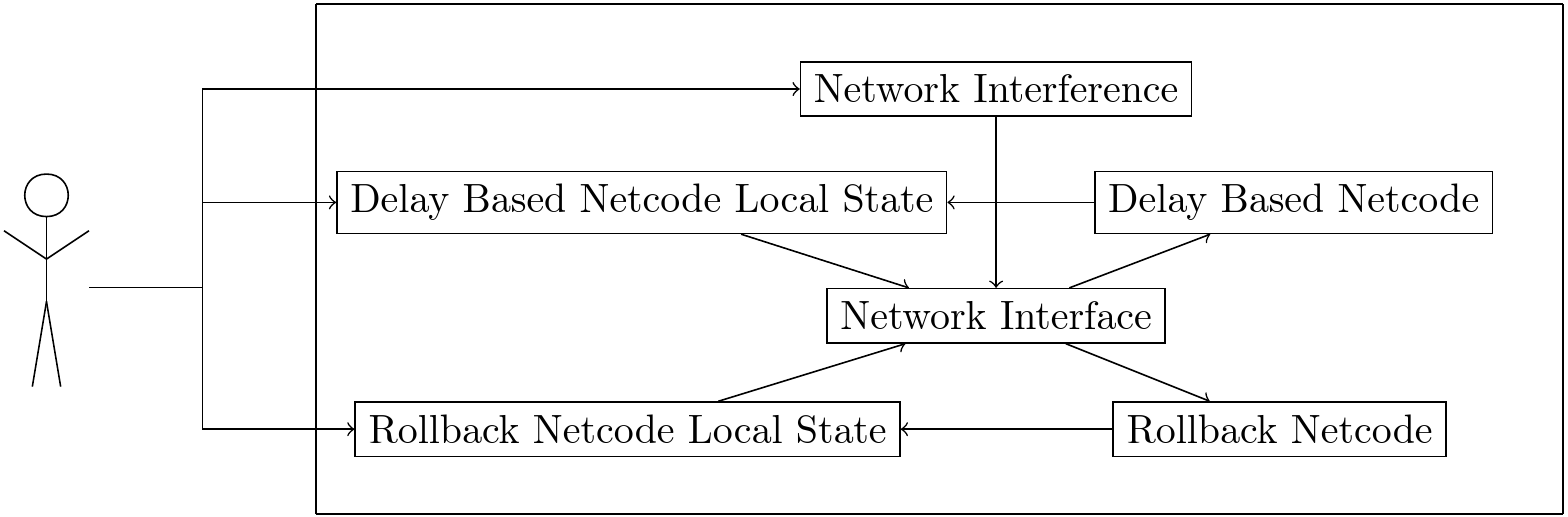
\includegraphics[width=\textwidth]{UIDesign}
\caption{Data Flow Diagram for Rollback Visualization tool}
\label{fig:DFD}
\end{figure}

\subsection{Implementation}

Initially the packet structure was chosen to be a single frame's input, however during development it was realized that the packet structure improvements mentioned in this document could be applied to combat packet loss.

State serialization was surprising simple, as the only two dynamic elements of the game were the two players. This meant that that the only properties to save were be the location and velocity of the avatars. More functionality, such as a health system, or audio effects, which are present in most modern games, extra systems would have had to be implemented on top to support dynamic saving and loading of game state.

Experiment With packet loss solutions


How seperate rendering from game state in unity? = Don't allow render texture to update


If a players inputs cannot change the state, then the simulation can continue without them. This can be used to slightly reduce the average amount of rollbacks and freezes in both netcode implementations. To implement this idea, a frames till actionable variable was added to the packet data, and the delay based netcode would not freeze for the remote user's inputs / rollback would not re-simulate frames if the guessed inputs were different whilst the frames till actionable value was larger than 0. This could also have further adaption in rollback netcode, where only a certain number of the remote's inputs could matter, minimizing potential rollbacks.


I noticed desyncs happening, between my adjacent simulations, despite inputs being identical. In order to try to fix this, I made more thorough re-jump detection, reducing parallelization in the code, manually ran physics updates for a set duration in stead of relying upon unity's fixed updates. Ultimately to no prevail. So I had to chose between redesigning unity's physics engine (the presumed source of lack of determinism) for deterministic behaviour or re-designing my visualization tool. I chose redeisgn as I could felt I could demonstrate the difference in delay based and rollback netcode from a users experience, if they were allowed to toggle between the different types of netcode.

reworked design

Networked state
 |                  \
\ /                  \
 V                    Netcode handler (recives input from game states and handles communication between them) - Network interfence customiser, Rollback, delay based, remote input
1 game states              
/             \                        \
1 local player   1 remote player        local input
 remote input subclass of local input

made own fixed size buffer class to prevent excess memory being used
Rollback always saving state, so if swap, can load prior states
Delay based code explained
Rollback code explained
pause game when rollbacks happen

having issues with frames taking longer than 16ms (Turns out unity overhead)
simulate max rollbacks 100\% of time
needed extra for game state from rollback explained

Buffer sizes?

Implement ideas from delay based netcode packet soultions = expanded packet size

\subsection{Evaluation}
Unity no determinism (redo engine?)
Rollback hard even for simple projects
Didn't implement Audio or particle systems
Better ping modelling
This simulation could also allow for testing of various improvements of the netcodes, such as multiple packet sending, increasing frames sent, etc.

\section{Improvements for Rollback}



\subsection{Prediction Quality}
https://www.diva-portal.org/smash/record.jsf?pid=diva2%3A1560069&dswid=-2962  -> neural networks

-Naive is ~90\% accurate {https://www.youtube.com/watch?v=k9JTIn1SVQ4\&t=1888s}
hard to run expensive algorithms alongside large rollbacks (cite MKX talk)

\subsection{Packet Contents Optimization}
Delay based strategies
How many frames to send, request for frame? = delay frames? + constant?

I propose a theory for rollback frames 
\[rollback frames = ceiling{max acceptable ping}{2*frameduration} - delay frames)\]
for dynamic: dynamically changing rollback = minimal effect, (Problem with maxing rollback? = Divergence and hardware doesn't support rolling back that far in 1 frame (16ms))
however try to keep delay static \cite{sec:Industry Issues}

\subsection{Input Locking}
No need for rollbacks when input doesn't matter, i.e. hit stun, hit pause, cutscene, jumping, in a move past a cancel window \cite{sec:Industry Issues}

\subsection{Conclusion}

Multiplayer online games have continued to gain popularity over the last few years as the growth and capacity of the internet has increased. Games involving fight simulations require highly responsive interaction with the local user. A number of techniques have been explored in this paper to achieve this goal over a network with latency. The primary strategy 'rollback netcode' uses prediction to overcome the limitations of network latency. This solution can be difficult to implement in pre-existing games but the availability of open source software to support rollback netcode has made implementation easier. Games that are originally developed with rollback in mind are easier to design and implement.

\section{Conclusions and further work}

Overall rollback hard to implement, but not impossible, newer games not releasing without it. Lessons learnt. Probably not applicable for wider use case. 

furture work: 
Non-game applications? Expand upon demo
\begin{thebibliography}{25}

\bibitem{GGPODocumentation} {\texttt https://drive.google.com/file/d/1nRa3cRBQmKj0-SEyrT\_1VNOkPOJWNhVI/view} or 
{\texttt https://web.archive.org/web/20220101162600/https://drive.google.com/file/d/1nRa3cRBQmKj0-SEyrT\_1VNOkPOJWNhVI/view} 
Tony C., GGPO Game Developer Magazine's article. 2012. (Visited 25/05/2022)

\bibitem{FGCMajors} {\texttt https://liquipedia.net/fighters/Tier\_1\_Tournaments} or 
{\texttt https://web.archive.org/web/20210121113554/https://liquipedia.net/fighters/Tier\_1\_Tournaments} 
Liquidpedia list of major fighting game tournaments. (Visited 25/05/2022)

\bibitem{FirstUSTournament} {\texttt https://www.usgamer.net/articles/the-oral-history-of-evo} or 
{\texttt https://web.archive.org/web/20220321000753/https://www.usgamer.net/articles/the-oral-history-of-evo} 
John L., The Oral History of EVO: The Story of the World's Largest Fighting Game Tournament (Visited 25/05/2022)

\bibitem{FGCAsEsport} {\texttt https://esportsinsider.com/2021/10/can-fighting-games-become-a-mainstream-esport/} or 
{\texttt https://web.archive.org/web/20220516060805/https://esportsinsider.com/2021/10/can-fighting-games-become-a-mainstream-esport/} 
Elizbar R., Can fighting games become a mainstream esport without abandoning grassroots?. (Visited 26/02/2022) 

\bibitem{SmashTournamentsInThePandemic} {\texttt https://www.ssbwiki.com/COVID-19\_pandemic\_and\_its\_impact\_on\_competitive\_Smash} or {\texttt https://web.archive.org/web/20220516020551/https://www.ssbwiki.com/COVID-19\_pandemic\_and\_its\_impact\_on\_competitive\_Smash} List of smash tournaments affected by the pandemic. (Visited 26/02/2022) 

\bibitem{GuiltyGearStriveInThePandemic} {\texttt https://techraptor.net/gaming/opinions/guilty-gear-strive-changed-fighting-games-rollback-netcode} or {\texttt https://web.archive.org/web/20210713144527/https://techraptor.net/gaming/opinions/guilty-gear-strive-changed-fighting-games-rollback-netcode} Davi B. Guilty Gear Strive Might Have Changed Fighting Games Forever. (Visited 26/02/2022)

\bibitem{DelayVsRollback} {\texttt https://arstechnica.com/gaming/2019/10/explaining-how-fighting-games-use-delay-based-and-rollback-netcode/} or {\texttt https://web.archive.org/web/20220425211823/https://arstechnica.com/gaming/2019/10/explaining-how-fighting-games-use-delay-based-and-rollback-netcode/} Ricky P. Explaining how fighting games use delay-based and rollback netcode. (Visted 26/05/2022)

\bibitem{BadNetcode} {\texttt https://www.polygon.com/2020/3/25/21192522/netcode-samurai-showdown-fighting-games-rollback-delay} or {\texttt https://web.archive.org/web/20220401231646/https://www.polygon.com/2020/3/25/21192522/netcode-samurai-showdown-fighting-games-rollback-delay} David C. Bad netcode is killing many of your favorite fighting
games. (Visted 26/05/2022)

\bibitem{RollbackDevelopment} {\texttt https://gamasutra.com/view/news/34050/Interview\_How\_A\_Fighting\_Game\_Fan\_Solved\_Internet\_Latency

\_Issues.php} or {\texttt https://web.archive.org/web/20220325062609/https://gamasutra.com/view/news/34050/
Interview\_How\_A\_Fighting\_Game\_Fan\_Solved\_Internet\_Latency\_Issues.php} Kyle O. Interview: How A Fighting Game Fan Solved Internet Latency Issues. (Visted 26/05/2022)

\bibitem{FightingGameDefine} {\texttt https://archive.org/details/nextgen-issue-015/page/n33/mode/2up} "The Next Generation 1996 Lexicon A to Z: Fighting Game". (Visited 26/05/2022)

\bibitem{DelayBasedNetcode} {\texttt https://www.gamasutra.com/view/feature/3094/1500\_archers\_on\_a\_288\_network\_.php} or {https://web.archive.org/web/20220506231117/https://www.gamasutra.com/view/feature/3094/
1500\_archers\_on\_a\_288\_network\_.php} Mark T. 1500 Archers on a 28.8: Network Programming in Age of Empires and Beyond. (Visted 26/05/2022)

\bibitem{FightingGameNetworking} {\texttt https://web.archive.org/web/20210228051849/https://mauve.mizuumi.net/2012/07/05/understanding-fighting-game-networking.html} Mauve M. Understanding Fighting Game Networking. (Visted 26/05/2022)

\bibitem{GamesWithRollback} {\texttt https://attackofthefanboy.com/guides/rollback-netcode-games-list/} or {\texttt https://web.archive.org/web/20211122034207/https://attackofthefanboy.com/guides/rollback-netcode-games-list/} Andron S. Rollback Netcode Games List (March 2022). (Visted 26/05/2022)

\bibitem{SSBU} {\texttt https://en.wikipedia.org/wiki/Super\_Smash\_Bros.\_Ultimate} or {\texttt https://web.archive.org/web/20220519200835/https://en.wikipedia.org/wiki/Super\_Smash\_Bros.\_Ultimate} Super Smash Bros. Ultimate. (Visited 26/05/2022)

\bibitem{GBFV} {\texttt https://en.wikipedia.org/wiki/Granblue\_Fantasy\_Versus} or {\texttt https://web.archive.org/web/20220512125807/https://en.wikipedia.org/wiki/Granblue\_Fantasy\_Versus} Grandblue Fantasy Versus (Visited 26/05/2022)

\bibitem{UNI} {\texttt https://en.wikipedia.org/wiki/Under\_Night\_In-Birth} or {\texttt https://web.archive.org/web/20220516020108/https://en.wikipedia.org/wiki/Under\_Night\_In-Birth} Under Night In-birth (Visited 26/05/2022)

\bibitem{SamSho} {\texttt https://en.wikipedia.org/wiki/Samurai\_Shodown\_(2019\_video\_game)} or {\texttt https://web.archive.org/web/20220504020927/
https://en.wikipedia.org/wiki/Samurai\_Shodown\_(2019\_video\_game)} Samurai Shodown (Visited 26/05/2022)

\bibitem{SVI} {\texttt https://en.wikipedia.org/wiki/Soulcalibur\_VI} or {\texttt https://web.archive.org/web/20220421074040/https://en.wikipedia.org/wiki/Soulcalibur\_VI} Soulcalibur VI (Visited 26/05/2022)

\bibitem{DOA6} {\texttt https://en.wikipedia.org/wiki/Dead\_or\_Alive\_6} or {\texttt https://web.archive.org/web/20220130144906/https://en.wikipedia.org/wiki/Dead\_or\_Alive\_6} Dead or Alive 6 (Visited 26/05/2022)

\bibitem{UFC4} {\texttt https://en.wikipedia.org/wiki/EA\_Sports\_UFC\_4} or {\texttt https://web.archive.org/web/20211019192531/https://en.wikipedia.org/wiki/EA\_Sports\_UFC\_4} EA Sports UFC 4 (Visited 26/05/2022)

\bibitem{DBFZ} {\texttt https://en.wikipedia.org/wiki/Dragon\_Ball\_FighterZ} or {\texttt https://web.archive.org/web/20220424200258/https://en.wikipedia.org/wiki/Dragon\_Ball\_FighterZ} Dragon Ball FighterZ (Visited 26/05/2022)

\bibitem{Core-ARollback} {\texttt https://www.youtube.com/watch?v=0NLe4IpdS1w} or {\texttt https://web.archive.org/web/20220529231214/https://www.youtube.com/watch?v=0NLe4IpdS1w} Core A Gaming. Analysis: Why Rollback Netcode Is Better. (Visted 31/05/2022)

\bibitem{KIInterview} {\texttt https://www.youtube.com/watch?v=1RI5scXYhK0} or {\texttt https://web.archive.org/web/20220330062542/https://www.youtube.com/watch?v=1RI5scXYhK0} Hold Back To Block. Talking Netcode With Adam "Keits" Heart (Visited 31/05/2022)

\bibitem{InputLatencyDatabase} {\texttt https://displaylag.com/video-game-input-lag-database/} or {\texttt https://web.archive.org/web/20220519183335/https://displaylag.com/video-game-input-lag-database/} Display Lag. Video Game Input Lag Database. (Visted 02/06/2022)

\bibitem{8Frames} {\texttt https://www.gdcvault.com/play/1025021/8-Frames-in-16ms-Rollback} or {\texttt https://web.archive.org/web/20210819020226/https://www.gdcvault.com/play/1025021/8-Frames-in-16ms-Rollback} Michael S. 8 Frames in 16ms: Rollback Networking in 'Mortal Kombat' and 'Injustice 2'. (Visted 08/06/2022)

\bibitem{Netcode 1} {\texttt https://www.eventhubs.com/news/2022/jan/09/3-problems-sf5-netcode/} Jon G. 3 major problems with Street Fighter 5's netcode I want fixed. (Visted 08/06/2022)

\bibitem{Netcode 2} {\texttt https://litetheironman.medium.com/street-fighter-v-and-rollback-netcode-101-8921a1e8a1c6} Nathan D. Street Fighter V and Rollback Netcode 101. (Visted 08/06/2022)

\bibitem{Netcode 3} {\texttt https://www.youtube.com/watch?v=iGgG6eWk1Xo} Brian F. Why SFV Netcode Sucks. (Visted 08/06/2022)

\bibitem{Netcode 4} {\texttt https://egmnow.com/street-fighter-v-has-finally-fixed-its-netcode-but-a-modder-did-it-first/} Dave M. Street Fighter V Has Finally Fixed Its Netcode—But a Modder Did It First. (Visted 08/06/2022)

\bibitem{SFV 1} {\texttt https://www.youtube.com/watch?v=OtSveL7X6xg} DigitalHalftones.  Altimor's SFV Netcode Fix Mod Visually Explained. (Visted 08/06/2022)

\bibitem{SFV 2} {\texttt https://www.youtube.com/watch?v=9ENocn-x0Ws} fluffysheap. SFV Netcode Fix. (Visted 08/06/2022)

\bibitem{SFV 3} {\texttt https://github.com/https://github.com/fluffysheap/SFVNetcodeFix/SFVNetcodeFix} fluffysheap. SFV Netcode Fix. (Visted 08/06/2022)

\end{thebibliography}
\end{document}
